\documentclass{article}
\usepackage{nips15submit_e,times}
\usepackage[hidelinks]{hyperref}
\usepackage{url}
\usepackage{graphicx}
\usepackage{booktabs}
\usepackage{amsmath,amssymb}

\title{Whom to Trust? Trust-Aware Delegation for\\Decentralized LLM-Agent Networks}

\author{
Adele Chinda (002831349) \quad\quad Trilok Padhi (002716700)\\
Group 21 \textperiodcentered{} CSC 8220 Task III \textperiodcentered{} Milestone 2 Progress Report \textperiodcentered{} Georgia State University
}

\nipsfinalcopy

\newcommand{\tada}{\textsc{Tada}}

\begin{document}
\maketitle
\vspace{-2.2em}

% =====================================================================
\section{Introduction}
PPAI~\cite{ppai} lets each user's edge agent delegate a query to a peer whose agent is more capable.
Queries and agents are matched in a shared prototype space, and a Bayesian load game picks a capable,
lightly loaded peer. PPAI, however, \emph{trusts every peer}: capability vectors are self-reported
and answers are accepted at face value. In our simulator, this makes it fragile. With 10\% of peers
lying about their skill, PPAI's accuracy falls from 0.73 to 0.19; with 10\% colluding on a shared
wrong answer, it falls to 0.04. We study \emph{trust-aware delegation}: whom to ask, how many peers
to ask, and how to combine their answers when some peers are adversarial and every verification
costs a network round trip. So far we have built a simulator grounded in PPAI's measured accuracies,
together with four baselines. We have also built \tada{} (Trust-Aware Delegation with Audits) and a
first Q-learning controller. With 30\% colluders, \tada{} keeps 0.77 accuracy, where Dawid--Skene and
majority voting fall to $\le$0.13 and EigenTrust reaches 0.64, and it sends 17\% fewer probes.

% =====================================================================
\section{Problem Statement and Formulation}
\textbf{System.} There are $n$ peers. Each query belongs to one of $K$ skill clusters (PPAI's
prototypes). Peer $j$ advertises a capability vector $r_j\in[0,1]^K$ and answers a cluster-$k$
query correctly with an unknown probability $a_{jk}$. Each peer is a FIFO server with rate $\mu_j$,
and a remote probe adds a delay $d$ in each direction. A query $q$ has a cluster $k_q$ and a true
answer $y_q\in\{1,\dots,L\}$ (multiple choice, $L=4$).
\textbf{Decision.} The owner's policy $\pi$ sends probe sets $S_1,S_2,\dots$ in rounds and waits for
each round's answers before deciding whether to stop. It then outputs $\hat y_q$. It may also send
\emph{audits}, i.e.\ gold questions with known answers. The objective is
\begin{equation}
\textstyle\max_\pi\ \mathbb{E}\big[\mathbb{1}\{\hat y_q=y_q\}\big]-\gamma\,\mathbb{E}\big[|S(q)|+A(q)\big]-\eta\,\mathbb{E}[T_q],
\end{equation}
where $|S(q)|$ counts probes, $A(q)$ counts audits, and $T_q$ is the end-to-end latency. There is no
trusted third party, no pre-trusted peer, and no ground truth beyond the audit pool.
\textbf{Threats.} A fraction $f$ of peers advertise $r_{jk}=0.95$ everywhere:
(T1)~\emph{skill liars} answer correctly with probability 0.15;
(T2)~\emph{colluders} all give the same wrong answer to each query;
(T3)~colluders \emph{whitewash}, re-joining under a fresh identity when their reputation drops below 0.4~\cite{whitewash};
(T4)~colluders \emph{camouflage} by answering correctly with probability 0.3.
For now, gold questions are assumed indistinguishable from user queries.
\textbf{Why AI.} Peer reliability is latent and must be inferred from noisy, correlated answers
(Bayesian inference, EM). Stopping is a sequential decision, i.e.\ a small MDP for reinforcement
learning. Choosing whom to audit is an exploration--exploitation (bandit) problem.

% =====================================================================
\section{Motivation}
\textbf{Interesting:} P2P trust is well studied for file sharing, where a download can be checked
against a hash. LLM answers have no hash. Honest peers are imperfect (accuracies of 0.13--0.87 in
PPAI's Table~I) and their errors are correlated, so disagreement is weak evidence of malice, while
a coalition can manufacture agreement. \textbf{Important:} open agent-to-agent networks are emerging,
a wrong medical or financial answer is costly, and PPAI lists trust as an open problem. Verification
also consumes network resources: each extra probe costs a round trip and GPU time. Deciding how much
to verify is therefore a networking resource-allocation problem, not only a security problem.

% =====================================================================
\section{Related Work}
\textbf{LLM routing and ensembles.} RouterDC~\cite{routerdc}, RouteLLM~\cite{routellm} and KABB~\cite{kabb}
route queries on one trusted platform. Self-consistency~\cite{selfconsistency} and ``More
Agents''~\cite{moreagents} show that aggregating answers helps, but they assume honest members.
PPAI~\cite{ppai} decentralises routing but keeps that assumption.
\textbf{P2P reputation.} EigenTrust~\cite{eigentrust} anchors global trust on pre-trusted peers.
PeerTrust~\cite{peertrust} and Beta reputation~\cite{betarep} aggregate feedback about transactions,
and surveys~\cite{marti2006,hoffman2009} catalogue whitewashing and Sybil attacks~\cite{sybil}. All of
these assume transaction outcomes are observable.
\textbf{Crowdsourced truth inference.} Dawid--Skene~\cite{dawidskene}, GLAD~\cite{glad} and
Karger et al.~\cite{karger2011} infer worker reliability without labels, but assume independent errors,
which collusion breaks. Gold questions~\cite{gold} inspire our audits.
\textbf{BFT and verifiable inference.} BFT~\cite{byzantine,pbft} needs deterministic replicas, whereas
honest LLMs legitimately disagree. zkLLM~\cite{zkllm} is far too slow for interactive queries.
\textbf{Gap:} we are not aware of work that combines latent-reliability inference with adaptive probe
allocation under collusion in a delay-sensitive network.

% =====================================================================
\section{Plan of Action}
\vspace{-0.4em}
\begin{center}
\small
\begin{tabular}{@{}lll@{}}
\toprule
When & Milestone & Lead\\
\midrule
Oct 13--21 & Simulator, baselines, \tada{}, first RL controller \emph{(done)} & Both / Adele\\
Oct 22--28 & Milestone 2 report and progress slides & Both\\
Oct 29--Nov 11 & Real answers of the 5 models (vLLM~\cite{vllm}); real traces~\cite{splitwise,burstgpt} & Trilok\\
Nov 12--25 & Better learned control (per-round credit, audit bandit); stronger attacks & Adele\\
Nov 26--final & Final experiments, IEEE final report ($\ge$6 pages), 25-min talk & Both\\
\bottomrule
\end{tabular}
\end{center}
\vspace{-0.4em}
\textbf{Division of work.} T.~Padhi proposed the core direction of modelling peer disagreement to
assign trust. He leads threat models, the literature review, data pipelines and evaluation. A.~Chinda
leads the simulator, \tada{} and the RL controller. Both of us write and present.

% =====================================================================
\section{Research Progress}
\textbf{Simulator and data.} We built a discrete-event simulator with Poisson arrivals, FIFO peer
queues and network delay. Policies are written as processes that send probes and wait for the
replies. It has 50 peers, each an instance of one of PPAI's five agents (Qwen2.5-7B,
DeepSeek-R1-Distill-7B, Nemotron-Code-7B, HuatuoGPT-o1-7B, Llama-3-8B). Their accuracies on MMLU,
GSM8K, MedQA, ARC-C and AGIEval are taken from PPAI's Table~I, plus per-peer noise. Honest errors
fall on a shared distractor with probability 0.5, so they are correlated. Other settings: service
rates of 15--25/s, a one-way delay of 5\,ms, an arrival rate $\lambda=50$/s, 5000 queries per run,
and 5 seeds. \textbf{Baselines:} PPAI's argmax; majority vote over the 5 most ``relevant'' peers;
Dawid--Skene EM; and EigenTrust, which we give 3 pre-trusted honest peers (\tada{} gets none).

\textbf{\tada{}.} Per query, it
(1)~shortlists peers by reported relevance (PPAI's scoring stage);
(2)~ranks them by \emph{estimated} accuracy $\hat a_{jk}$ minus a load penalty, so lying about skill buys nothing;
(3)~asks the top 3 and, if the posterior of the best answer is below $\tau=0.9$, asks 2 more; and
(4)~with probability 0.15, sends a gold question from PPAI's own per-prototype question set $Q_k$ to a
peer it just used or to the peer whose audit record is most uncertain.
Each peer keeps Beta counts per cluster~\cite{betarep} for agreement, $(\alpha_{jk},\beta_{jk})$, and
for audits, $(g^+_{jk},g^-_{jk})$. Agreement may never claim more than the audit record supports:
\begin{equation}
\hat a_{jk}=\min\big\{\tfrac{\alpha_{jk}}{\alpha_{jk}+\beta_{jk}},\ U(g^+_{jk},g^-_{jk}),\ U(g^+_{j\cdot},g^-_{j\cdot})+\delta\big\},\quad
U=\hat p+z\sqrt{\hat p(1-\hat p)/(n+1)},
\end{equation}
where $\hat p$ and $n$ are the audit success rate and audit count, and the last term pools a peer's
audits over all clusters. Answers are combined with the one-coin posterior
$P(y{=}\ell\mid x_S)\propto\prod_{j\in S}\hat a_{jk}^{\mathbb{1}[x_j=\ell]}\big(\tfrac{1-\hat a_{jk}}{L-1}\big)^{\mathbb{1}[x_j\ne\ell]}$.
\textbf{Anchored agreement:} agreement counts are updated only if the same answer still wins
(posterior $\ge0.5$) when each peer is weighted by its \emph{audit-only} lower bound, floored at chance.
Unaudited colluders then carry no weight and cannot bootstrap their own trust.

\begin{figure}[t]
\centering
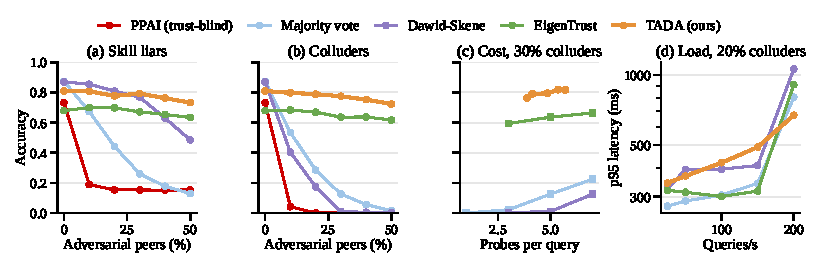
\includegraphics[width=\textwidth]{figures/summary.pdf}
\vspace{-1.7em}
\caption{(a,b)~Accuracy as the share of adversarial peers grows. (c)~Accuracy vs.\ probes per query
(committee size or $\tau$ swept). (d)~p95 latency vs.\ arrival rate. Means over 5 seeds.}
\label{fig:main}
\vspace{-0.5em}
\end{figure}

\begin{table}[t]
\centering
\small
\setlength{\tabcolsep}{3.4pt}
\caption{Accuracy with 30\% adversaries of each kind; probes and p95 latency are measured with
colluders. The rows marked $-$ remove one \tada{} component.}
\label{tab:abl}
\begin{tabular}{@{}lccccccc@{}}
\toprule
Method & No attack & Liars & Colluders & +Whitewash & +Camouflage & Probes & p95 (ms)\\
\midrule
\tada{} (full) & 0.81 & \textbf{0.79} & \textbf{0.77} & \textbf{0.75} & \textbf{0.76} & 4.2 & 376\\
\quad $-$ anchoring & 0.82 & 0.78 & 0.63 & 0.47 & 0.67 & 4.1 & 370\\
\quad $-$ audits & 0.76 & 0.57 & 0.42 & 0.42 & 0.61 & 4.8 & 432\\
\quad $-$ pooled audit cap & 0.81 & 0.79 & 0.76 & 0.74 & 0.76 & 4.2 & 373\\
\quad $-$ sequential (ask 5 at once) & 0.82 & 0.79 & 0.77 & 0.75 & 0.76 & 5.1 & 276\\
\midrule
EigenTrust ($m{=}5$) & 0.68 & 0.67 & 0.64 & 0.67 & 0.66 & 5.0 & 301\\
Dawid--Skene ($m{=}5$) & \textbf{0.87} & 0.77 & 0.01 & 0.01 & 0.34 & 5.0 & 333\\
Majority vote ($m{=}5$) & \textbf{0.87} & 0.26 & 0.13 & 0.13 & 0.31 & 5.0 & 268\\
\bottomrule
\end{tabular}
\vspace{-0.9em}
\end{table}

\textbf{Initial findings.}
(1)~PPAI is captured by any liar. Dawid--Skene handles independent liars but collapses under collusion
(0.01), because colluders look like a reliable majority (Fig.~\ref{fig:main}a,b).
(2)~\tada{} reaches 0.77 with 30\% colluders and 0.72 with 50\% (EigenTrust: 0.64 and 0.62), without
any pre-trusted peers. Only 4\% of the answers it uses come from adversaries, and it survives
whitewashing and camouflage. Accuracy climbs from 0.53 to 0.83 within the first 30\% of a run.
(3)~Audits and anchoring do the work (Table~\ref{tab:abl}): without audits, accuracy under collusion is
0.42; without anchoring, 0.63 (0.47 under whitewashing). The pooled audit cap adds little.
(4)~Verification costs the network. Sequential rounds save 18\% of probes but raise p95 latency from
276 to 376\,ms. Under heavy load the saved probes pay off: at 200 queries/s, \tada{} has the lowest
p95 latency (672\,ms vs.\ 804--1062\,ms; Fig.~\ref{fig:main}d).
(5)~The price of scepticism: with no attack, \tada{} is 6 points below a full 5-peer vote.
\textbf{Preliminary RL.} Tabular Q-learning~\cite{qlearning} replaces $\tau$. The state is (confidence,
round, load, cluster), the actions are \{stop, ask 2 more\}, and the reward is correctness minus costs
per probe and per second of latency. It is trained in simulation on seeds separate from the evaluation
seeds. With 30\% colluders at 150 queries/s, it learns to stop earlier: p95 latency falls from 576 to
310\,ms and probes from 4.3 to 3.3, for $-$1.4 accuracy points. Without the latency penalty it matches
the best threshold (0.79) but does not beat it; binary rewards are noisy.

\textbf{Challenges and how we addressed them.}
(a)~Our first answer model never let wrong answers agree, which made voting look almost perfect. We
switched to a shared-distractor multiple-choice model.
(b)~Agreement-only trust was captured by colluders (0.003 accuracy). Capping trust by audits fixed the
steady state, and anchoring fixed the warm-up (+14 points).
(c)~Our first queue model reserved servers for future verification rounds, producing spurious 12\,s
latencies. We rebuilt the simulator as a discrete-event simulation.
(d)~Asking one peer first caused up to 3 sequential rounds. Asking 3 first caps a query at two rounds
and cuts p95 latency by about 25\%.
\textbf{Next algorithms:} per-round credit assignment for the RL controller; a contextual bandit for
choosing whom to audit, with an adaptive audit rate; collusion detection from answer correlations;
adversaries that try to spot gold questions, and Sybil swarms; and real per-question model answers in
place of the synthetic model. Code, tests and the script that regenerates every number are attached.

{\small
\bibliographystyle{unsrt}
\bibliography{references}
}

\end{document}
